\documentclass[11pt]{report}
\usepackage{outline}
\usepackage{pmgraph}
\usepackage[normalem]{ulem}
\usepackage{graphicx}
\usepackage{listings}
\usepackage{caption}
\usepackage{dsfont}
\usepackage{indentfirst}
\newcommand\independent{\protect\mathpalette{\protect\independenT}{\perp}}
\def\independenT#1#2{\mathrel{\rlap{$#1#2$}\mkern2mu{#1#2}}}
\usepackage{amsmath}
\usepackage{amssymb}
\usepackage{amsfonts}
\title{\textbf{Lecture 11}}
\author{Meera Nanda, Varun Narayan, Romane d'Oncieu \\Chenyu Zhang, Hao Rong.}
\date{\oldstylenums{10}/\oldstylenums{02}/\oldstylenums{18}}
%--------------------Make usable space all of page
\setlength{\oddsidemargin}{0in}
\setlength{\evensidemargin}{0in}
\setlength{\topmargin}{0in}
\setlength{\headsep}{-.25in}
\setlength{\textwidth}{6.5in}
\setlength{\textheight}{8.5in}
%--------------------Indention
\setlength{\parindent}{1cm}

\begin{document}
%--------------------Title Page
\maketitle
\renewcommand{\chaptername}{}
\renewcommand{\thechapter}{}
\renewcommand{\thesection}{}
\renewcommand{\thesubsection}{}

 
%--------------------Begin Outline
\section{Recap}
\subsection{Curse of dimensionality :}
Data gets sparser and sparser as we get more data (larger dimensions).

\begin{figure}[ht]
    \centering
    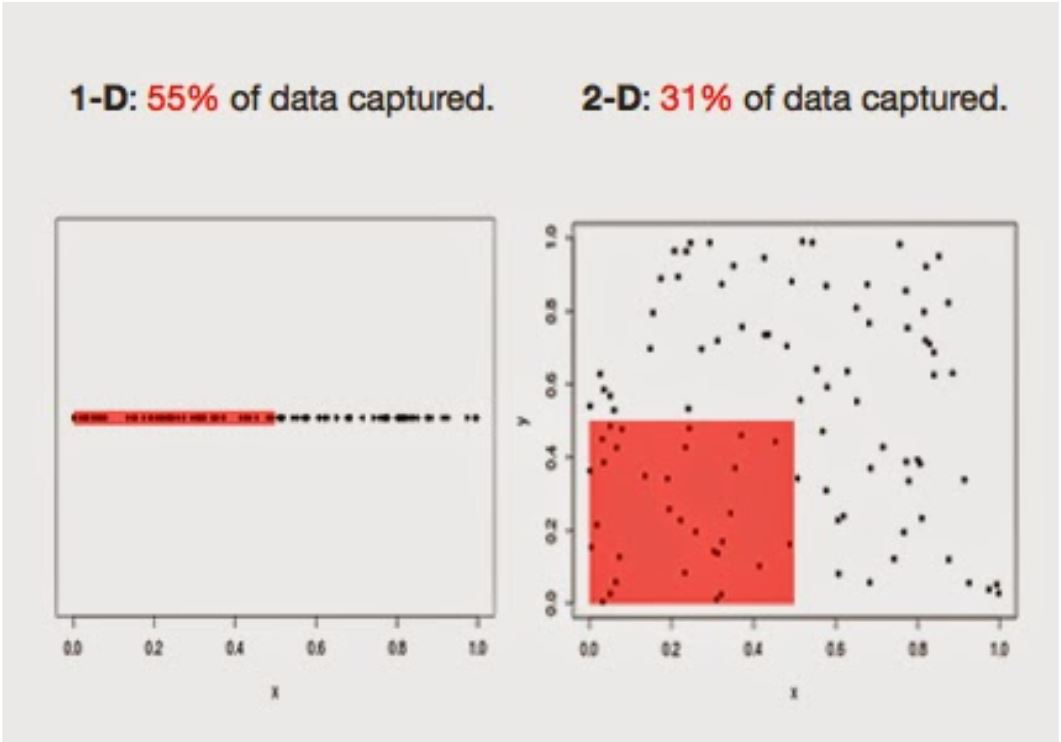
\includegraphics[width=0.4\linewidth]{image_1.JPG}
    \captionsetup{labelformat=empty}
\end{figure}

\subsection{Naive Bayes :}
We make the naive assumption that individual features are independent of one another given label value.

We can write this in 2 ways : 

- mathematically : $X_j \independent X_k | Y $ for $j\neq k$

- or just saying that the conditional density factorizes : 
\[f_j(X)=\prod_{k=1}^{p} f_{jk}(X_k)\]

Here $f_j$ is the conditional density of $X|Y=j$ and $f_{jk}$ is the conditional density of $X_k | Y=j$

The idea behind naive bayes is that when we look at a particular class, the features are independent. For example, when we look at the class "Female" or "Male", the features height and weight are independent within each class. Therefore, Naive Bayes enables us to work in only one dimension. 

\begin{figure}[ht]
    \centering
    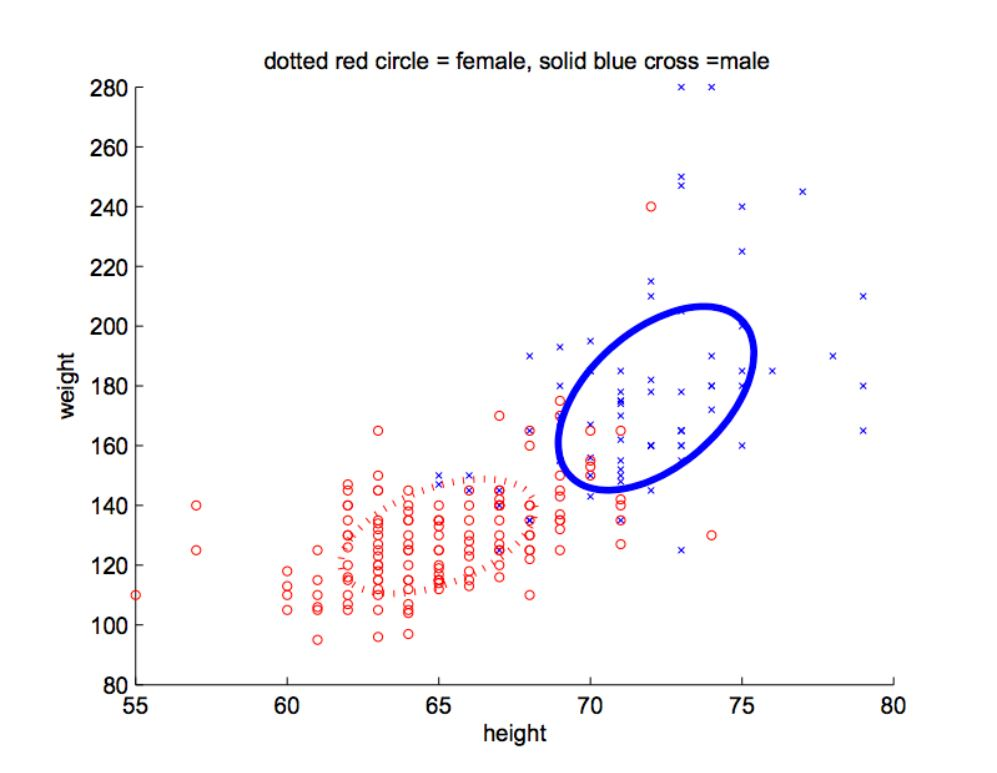
\includegraphics[width=0.5\linewidth]{image_2.JPG}
    \captionsetup{labelformat=empty}
\end{figure}


\subsection{Naive Bayes Classifier :} 
The idea is to estimate the $f_{jk}(X_k)$ for all k and then plug them in. 

For any instance, if we look at the log ratio we have : 
\[log \left(\frac{\hat{P}(Y=j|X)}{\hat{P}(Y=l|X)}\right) = log \left( \frac{\hat{\pi}_j}{\hat{\pi}_l}\right)+\sum\limits_{k=1}^p log \left(\frac{\hat{f}_{jk}(X_k)}{\hat{f}_{lk}(X_k)} \right)\]

As seen earlier in this course, if $Y=\left\{0 , 1\right\}$, $log \left(\frac{P(Y=j|X)}{P(Y=l|X)}\right) = logit\left[P(Y=1|X)\right]$.

For class frequencies, we can use empirical frequencies :
\[\hat{\pi}_j=\frac{\sum\limits_{i=1}^n \mathds{1}\left[Y_i=j\right] }{n}\]

\textbf{For discrete features :}

we can estimate the density functions:
\[\hat{f_{jk}}{(X_k)}=\frac{\sum\limits_{i=1}^n \mathbb{I}\left[Y_i=j , X_{ik}=x_k \right] +\alpha}{\sum\limits_{i=1}^n \mathbb{I}\left[Y_i=j\right] +\alpha}\]

We add the $\alpha$ to pad the data. If $\alpha=0$, we have the empirical frequencies and if $\alpha > 0$, we say we have \textbf{laplace smoothing}.\\


\textbf{For Continuous Features : }

We have several options: \\

\textbf{Option 1: Histogram Estimates} - bin the data and treat it as discrete features as above.\\

\textbf{Option 2: Kernel density estimate (KDE)}
\[\hat{f}_{jk}(x_k)=\frac{\sum\limits_{i=1}^n \mathbb{I}\left[Y_i=j\right] \varphi \left(\frac{x_k - X_{ik}}{\lambda}\right)}{\lambda \sum\limits_{i=1}^n \mathbb{I}\left[Y_i=j\right]}\]

\textbf{Option 3: Parametric density estimate} - we can recall this using an example of steps to follow :\\

- assume ${f}_{jk}(X_k)=\varphi \left(\frac{X_k - \mu}{\sigma}\right)$ \\

- estimate $\hat{\mu}$ and $\hat{\sigma}$ as sample mean and standard deviation\\

- plug in : $\Hat{f}_{jk}(X_k)=\varphi \left(\frac{X_k - \hat{\mu}}{\hat{\sigma}}\right)$



\newpage
\section{Bag of words features (BOW)}

Bag of words is an approach used to featurize (i.e. make into a quantitative feature) text data. \\

Given texts $s_1,...s_n$, e.g. $s_1$ = "my dog likes your dog", we treat each instance of a string as a BOW, ignoring the order but remembering the counts. \\

$BOW(s_1)$ = \{"your", "likes", "my", "dog", "dog"\}

Note that the above is not an ordered list. \\

From here, make a dictionary of all the words present in all the given strings. \\

$$
D = \bigcup\limits_{i=1}^n BOW(s_i)
$$

And featurize each text by: \\

$X_{ij}$ = number of times that word $j$ appears in $s_i$, $\forall j \in D$ \\

Then $X_i$ (as a vector) will capture the overall nature of the text. \\

\begin{figure}[ht]
    \centering
    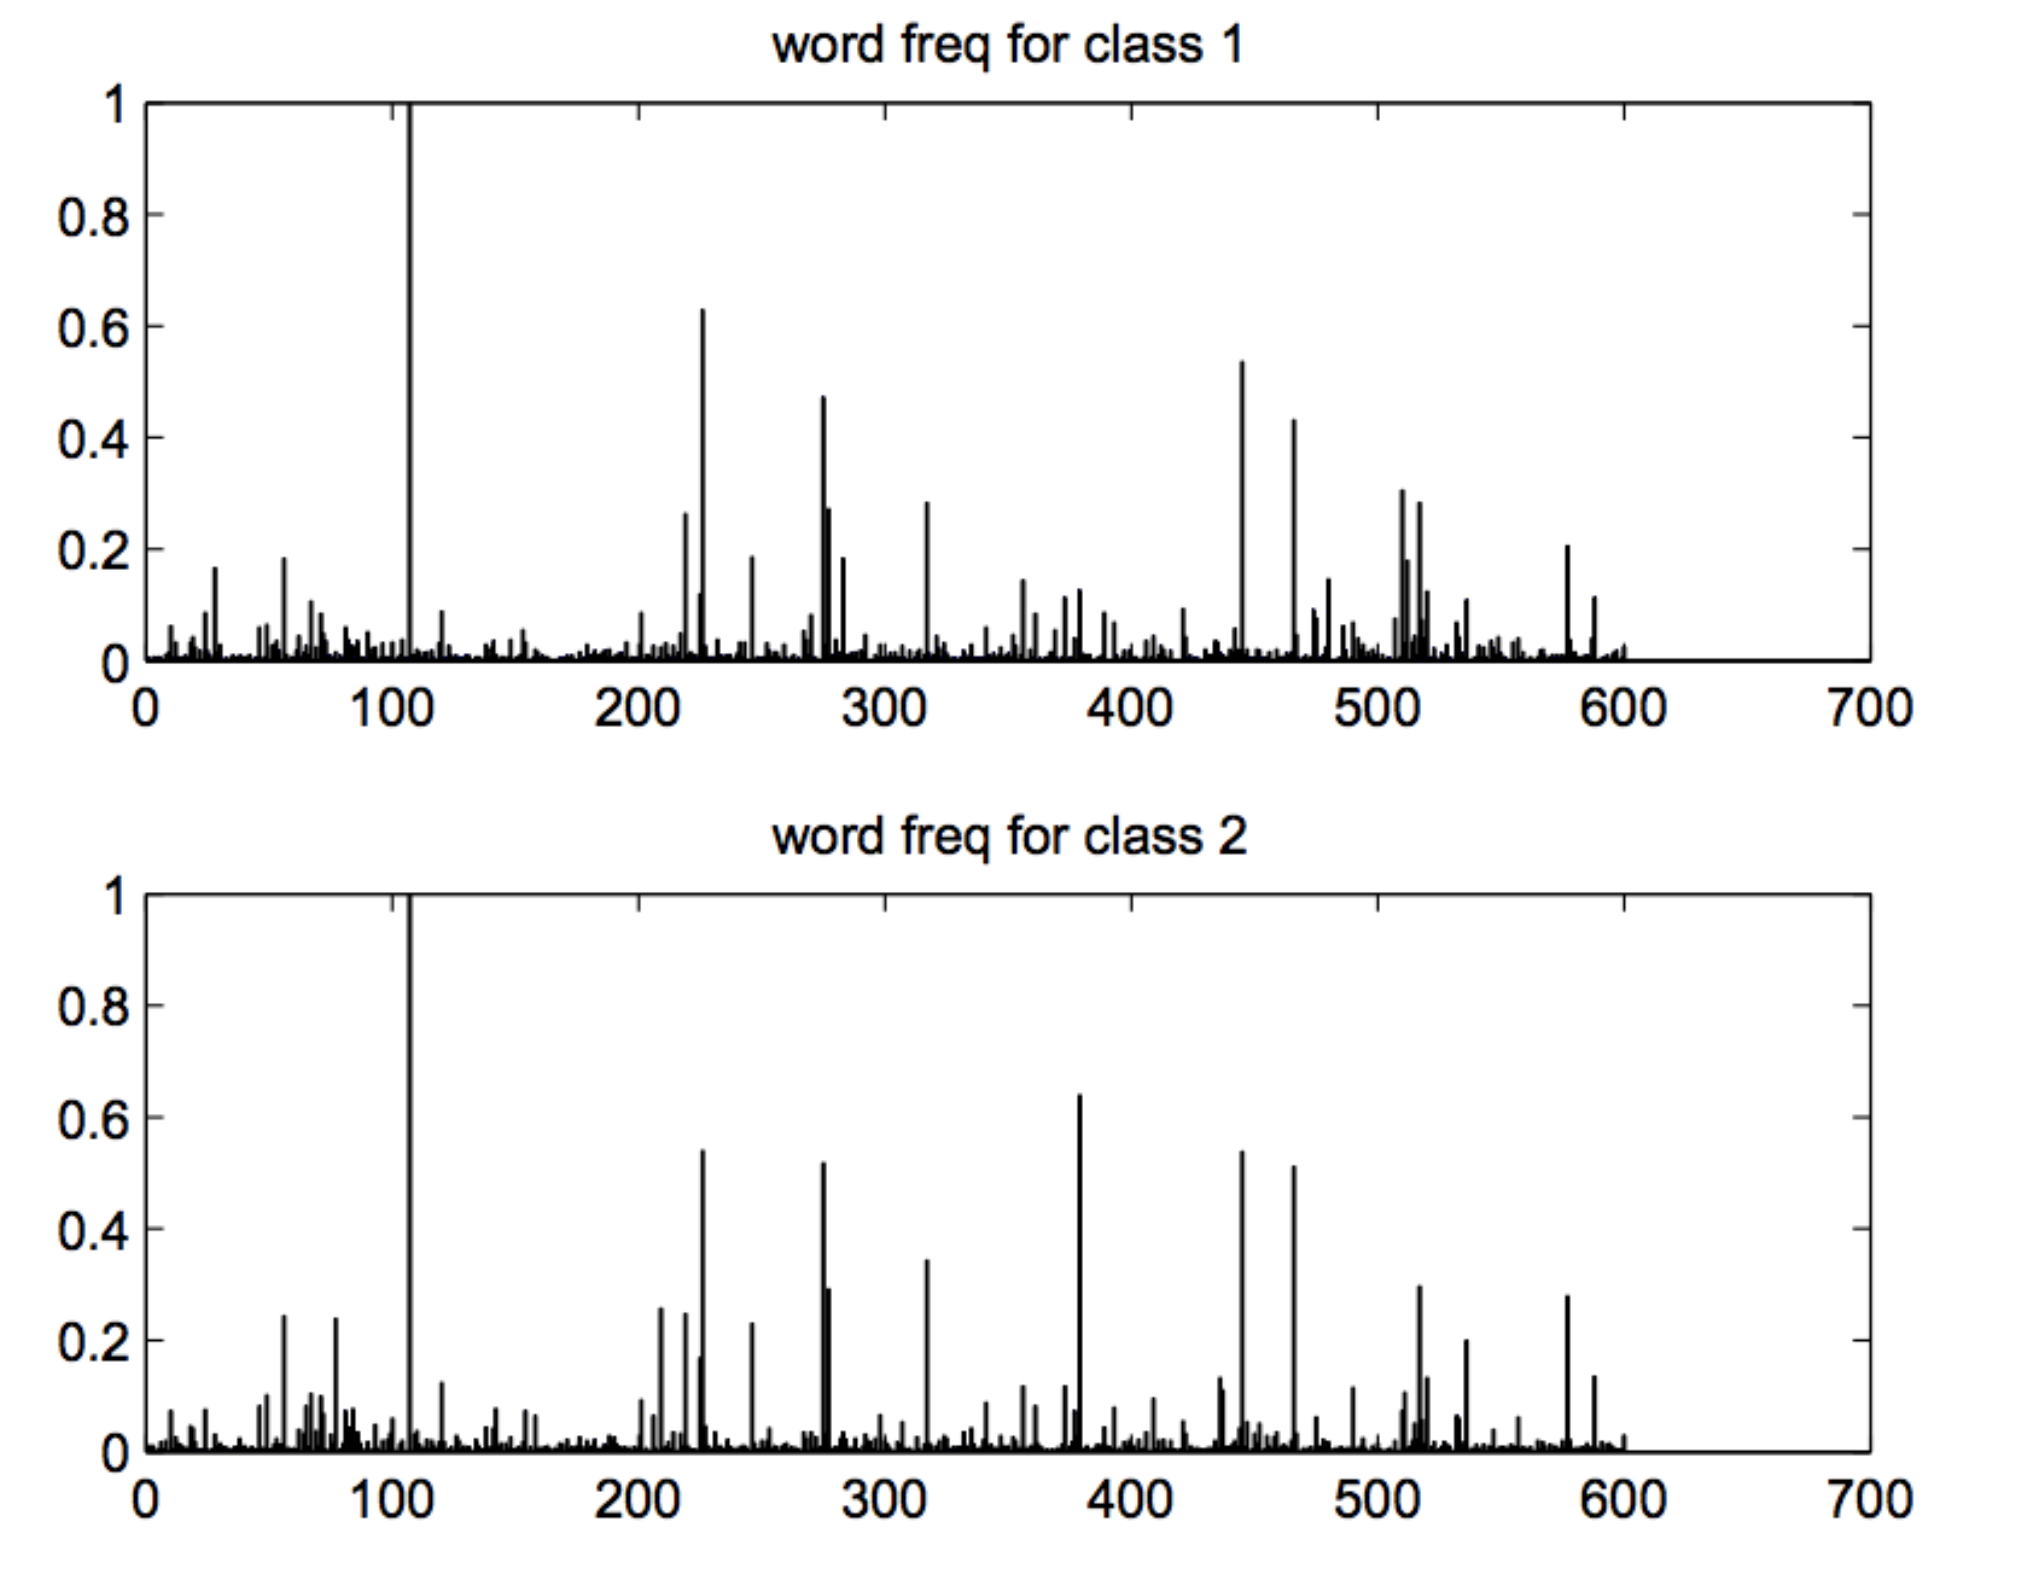
\includegraphics[width=0.8\linewidth]{image_4.png}
    \captionsetup{labelformat=empty}
\end{figure} 

\textbf{Important Considerations} \\

- Decapitalization: This form of preprocessing is used to ensure that the word "dog" and "Dog" are counted as the same feature. In this scenario, we are assuming that the capitalization of a word does not offer insight into the sentiment of text. This may not always be true however, for example if a review states that the food is "bad" versus "BAD", the latter is clearly a stronger sentiment. \\

- Lemmantization: This form of preprocessing returns the word to its root form. E.g. "likes" = "like". \\

- Pruning Contentless Words: Here you remove words such as "a" or "the" that do not change the meaning or sentiment of a text despite the number of times they appear. \\

- Normalization: The scores can also be normalized once tallied, however it is not required. There is no right or wrong approach in choosing to normalize the BOW. \\

- Ngrams: This process selects groups of words, potentially two at a time, to better capture the sentiment of a text. E.g. "my dog", "dog likes", etc. \\


\section{Naive Bayes with BOW}
BOW generates very high dimensional feature sets, which can be bad for the curse of dimensionality. However this process is perfect for implementing Naive Bayes. \\

First, try with $X_{ij} = \left\{0 , 1\right\}$ to see whether word $j$ appears within the text $i$. Then estimate the probability: \\

\[ \left({\hat{\mathbb{P}}(X_j=1|Y=k)}\right) = {\hat{P}_{jk}} =  \frac{\sum\limits_{i=1}^n \mathbb{I}[Y_i = k, X_ij = 1] + \alpha}{\sum\limits_{i=1}^n \mathbb{I}[Y_i = k] + \alpha}
\]
 
 This will produce an $\alpha$ smoothed fraction of k texts that have word j. \\
 
 Suppose $Y=\left\{0 , 1\right\}$, e.g. \{not spam, spam\}. Then using Naive Bayes: \\
 
 \[
 logit\left(\hat{\mathbb{P}}(Y=i|X)\right) = logit \left(\hat{\Pi}_1\right) + \sum\limits_{j}\left(X_j\log\left(\frac{\hat{P_{j1}}}{\hat{P_{j0}}}\right) + (1-X_j)log\left(\frac{1-\hat{P_{j1}}}{1-\hat{P_{j0}}}\right)\right)
 \]

Where $\Pi$ = how many things are spam, and $\Sigma$ is each word within the BOW. \\

If a word is more prevalent in one text, it is most likely a useful feature. It is also important to remember that BOW does not necessarily have to be just about words; the same concept can be applied to textons, e.g. groups of pixels in a picture. In the below image, we can see that it is being used to featurize groups of pixels in order to determine the texture represented.\\

\begin{figure}[ht]
    \centering
    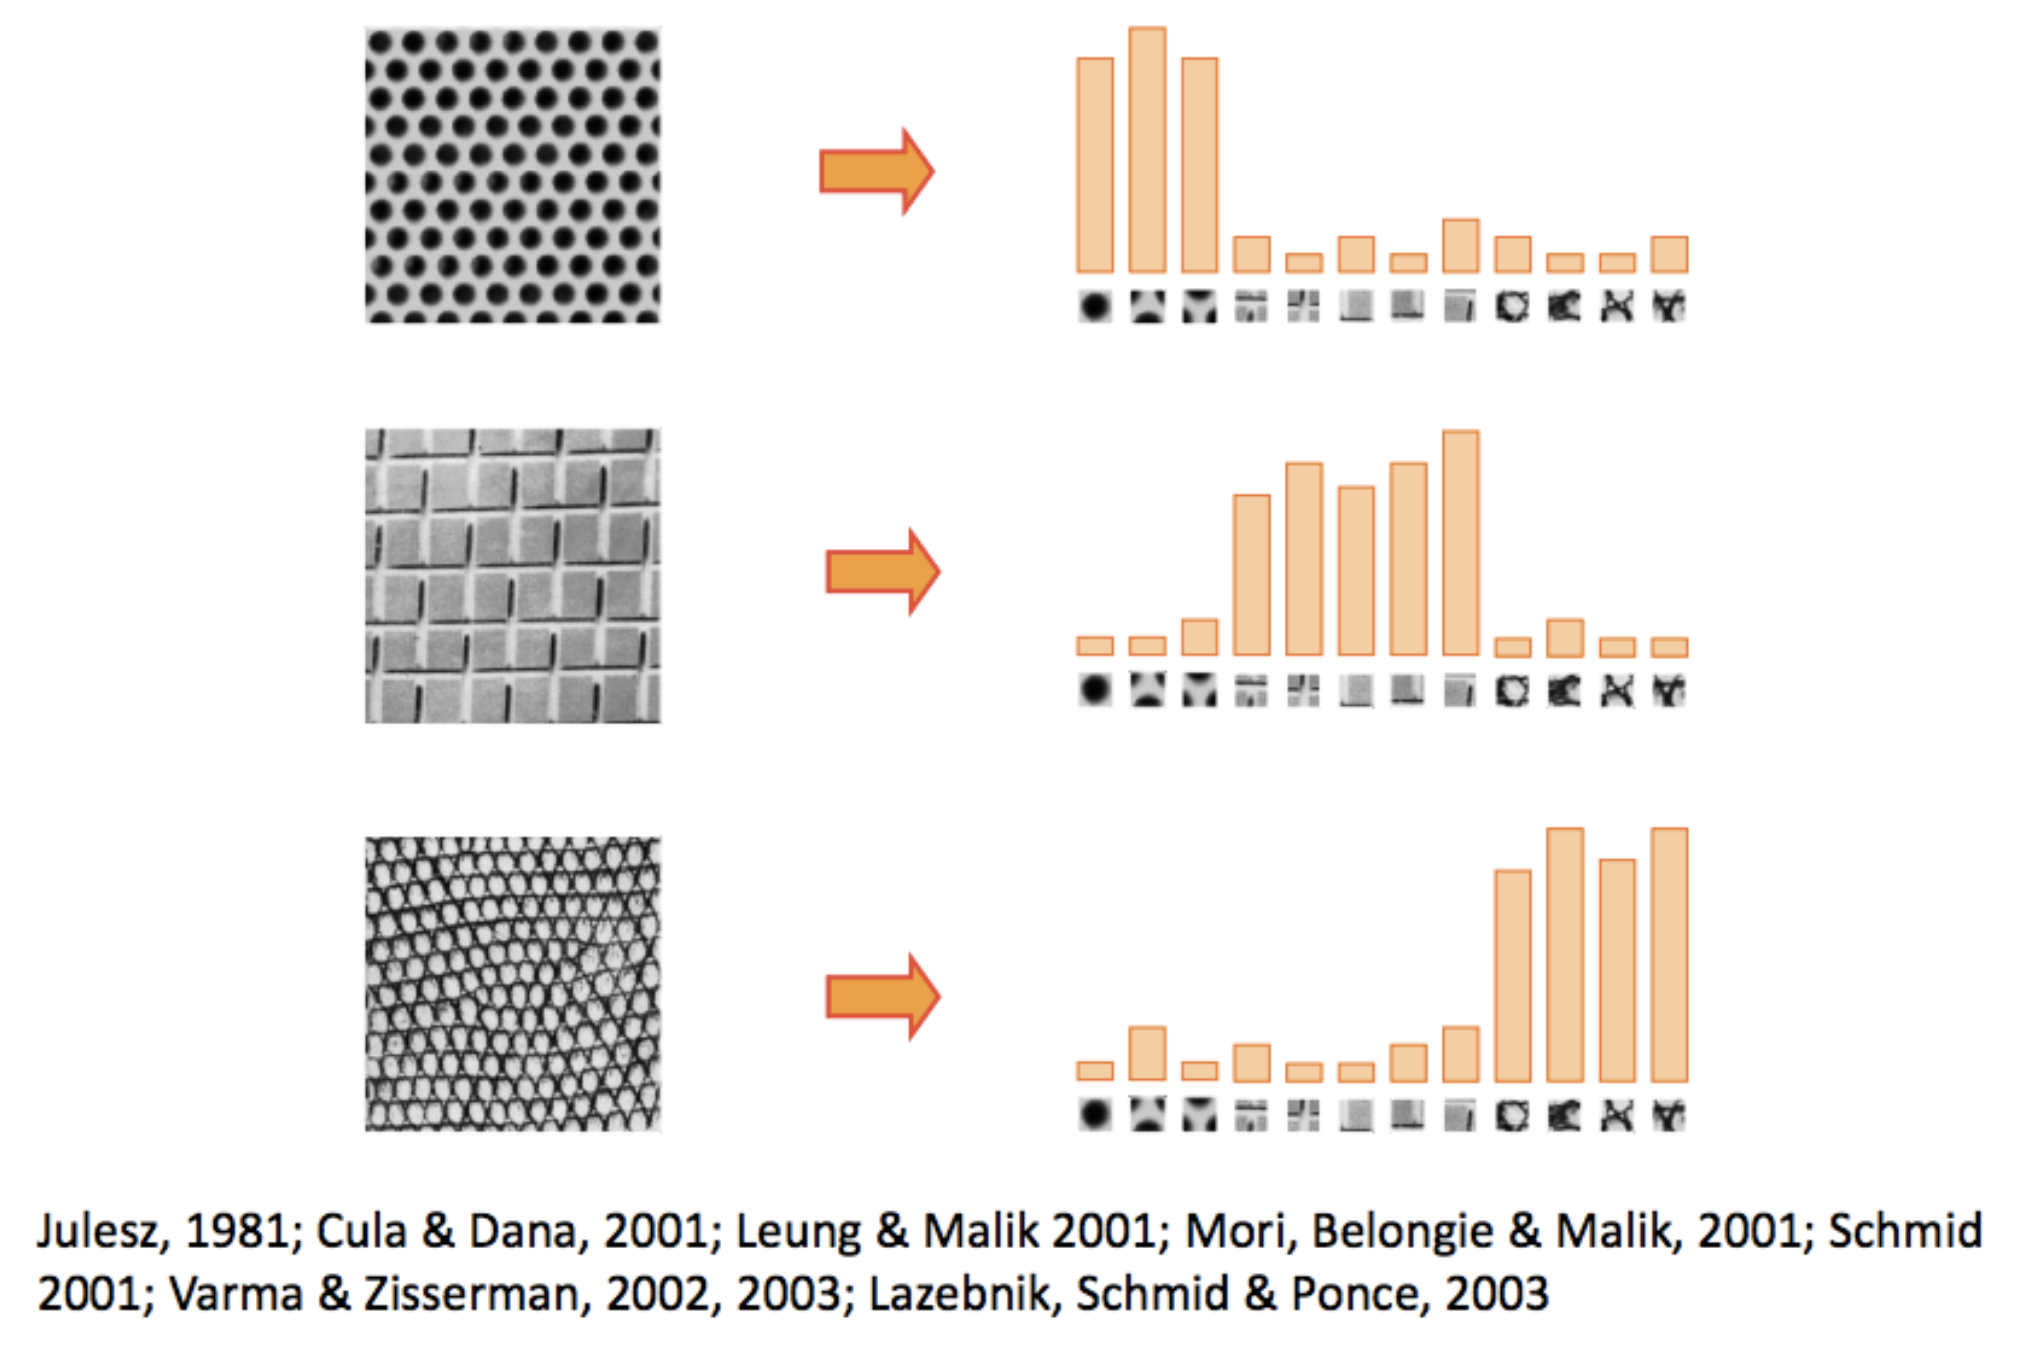
\includegraphics[width=1.0\linewidth]{image_3.png}
    \captionsetup{labelformat=empty}
\end{figure}

\newpage
\section{Eigen \& Singular Values Review}
For a square matrix $\mathbf{A} \in  \mathbb{R}^{p \times p}$ , 

$\lambda\in\mathbb{C}, \mathbf{V}\in\mathbb{R}^{p}$ are an eigen-value/eigen-vector pair of $\mathbf{A}$ if $\mathbf{AV}=\lambda\mathbf{V}$.  \\

If $\mathbf{A}$ is symmetric, $\mathbf{A} = \mathbf{A^T } \in\mathbb{R}^{p \times p}$, then all its eigenvalues are real. \\

Any square matrix can be diagonalized:
\[\mathbf{A} = \sum_{i=1}^{p} \lambda_i v_iv_i^T \]
\textit{s.t.} 
\[ v_i^T v_j=\begin{cases}
    1, & \text{if $i = j$}\\
    0, & \text{otherwise}
  \end{cases} \hspace{0.5cm}  \Rightarrow \text{Known as an ortho-normal set of vectors.}\]\\
\[\mathbf{A} = \mathbf{V \Lambda V^T}, \hspace{0.5cm} \Lambda= \begin{pmatrix}
\lambda_1  &      &      &   \hdots     &  0    \\
          & \lambda_2  &  &  &      \vdots   \\
          &      & \ddots &  &     \\
  \vdots        & & &\ddots &  \\
  0      &\hdots & & &\lambda_{p}
\end{pmatrix}, \hspace{0.5cm} \mathbf{V V^T}=\mathbb{I}=\mathbf{V^T V} \hspace{0.5cm}\]  
\[\Rightarrow \text{Known as an eigen-decomposition of } \mathbf{A} \text{where \textbf{A} is a real symmetric matrix} \]\\
If $\mathbf{A}$ is symmetric and\\

- all its eigenvalues are non-negative. $\mathbf{A}$ is called positive semi-definite (PSD) and we can define $\mathbf{A}^{1/2} = \mathbf{V\Lambda}^{1/2}\mathbf{V^T}$, 
\[\mathbf{\Lambda}^{1/2} = \begin{pmatrix}
\sqrt{\lambda_1}  &      &      &   \hdots     &  0    \\
          & \sqrt{\lambda_2}  &  &  &      \vdots   \\
          &      & \ddots &  &     \\
  \vdots        & & &\ddots &  \\
  0      &\hdots & & &\sqrt{\lambda_p}
\end{pmatrix}\]
$\mathbf{A}^{1/2}\mathbf{A}^{1/2} = \mathbf{V\Lambda}^{1/2}\mathbf{V^T}\mathbf{V\Lambda}^{1/2}\mathbf{V^T} = \mathbf{V\Lambda}\mathbf{V^T} = \mathbf{A}$\\

- all its eigenvalues are positive, $\mathbf{A}$ is called positive definite (PD)\

- all its eigenvalues are non-zero, $\mathbf{A}$ is called invertible/non-singular
\[\mathbf{A}^{-1} = \mathbf{V\Lambda}^{-1}\mathbf{V^T}\]
\[\mathbf{A}\mathbf{A}^{-1} = \mathbf{V\Lambda}^{-1}\mathbf{V^T}\mathbf{V\Lambda}^{-1}\mathbf{V^T} = \mathbb{I} = \mathbf{A}\mathbf{A}^{-1}\]

\newpage

\section{What about non-square matrices?}
In order to carry out SVD (singular value decomposition), the matrix doesn't need to be square. Any matrix can be SVD'd. For a rectangular matrix $A \in  \mathbb{R}^{p \times q}$, $\sigma \in \mathbb{R}$, $V \in  \mathbb{R}^{p}$ and $U \in  \mathbb{R}^{q}$ are a singular value, and left and right singular value, set of A if: \\
$$ AV = \sigma U $$
$$ A^T U= \sigma V $$

Take a non square matrix $A \in  \mathbb{R}^{p \times q}$ .
Let:
$$ A = \sum_{i=1}^{min(p,q)} \sigma_i u_iv_i^T \hspace{0.5cm}  \Rightarrow \hspace{0.5cm} \mathbf{A} = \mathbf{U \Sigma V^T}$$

\textit{s.t.} 
$$u_i^T u_j=\begin{cases}
    1, & \text{$i = j$}\\
    0, & \text{$i \neq j $}
  \end{cases} ,\hspace{1cm}
  v_i^T v_j=\begin{cases}
    1, & \text{$i = j$}\\
    0, & \text{$i \neq j $}
  \end{cases} $$ 
  
Where:
  $$
   \mathbf{U} \in \mathbb{R}^{p \times min(p,q)}, \hspace{1cm} \mathbf{V} \in \mathbb{R}^{q \times min(p,q)},\hspace{1cm} \mathbf{\Sigma} \in \mathbb{R}^{min(p,q) \times min(p,q)}$$
In Matrix for this can be seen as:
$$\mathbf{\Sigma} =
\begin{pmatrix}
\sigma_1  &      &      &   \hdots     &  0    \\
          & \sigma_2  &  &  &      \vdots   \\
          &      & \ddots &  &     \\
  \vdots        & & &\ddots &  \\
  0      &\hdots & & &\sigma_{min(p,q)}

\end{pmatrix}, \hspace{1cm} \mathbf{U^T U} = \mathbb{I}, \hspace{1cm} \mathbf{V^T V} = \mathbb{I}
$$

Note: $ \mathbf{A^T A} = \mathbf{V \Sigma U^T U \Sigma V^T} = \mathbf{V \Sigma^2 V^T}$ and $\mathbf{A A^T} = \mathbf{U \Sigma V^T V \Sigma U^T} = \mathbf{U \Sigma^2 U^T}$

Eigenvals of $\mathbf{A}^T\mathbf{A}$ are squared singular vals of \textbf{A} and eigenvectors of $\mathbf{A}^T\mathbf{A}$ are the left singular vectors of \textbf{A}

\section{An optimization view of SVD}

\subsection{Optimization}

Suppose we now have a matrix $\mathbf{M} \in \mathbb{R}^{n \times p}$.

We want to find $\mathbf{A} \in \mathbb{R}^{n \times r}$, $\mathbf{B} \in \mathbb{R}^{p \times r}$ for $r < n, p$, s.t. $\mathbf{AB}^T$ is closest to $\mathbf{M}$.

What's "closest"? In other words, we need to minimize the following:

$$
\min_{\substack{\mathbf{A} \in \mathbb{R}^{n \times r}\\{\mathbf{B} \in \mathbb{R}^{p \times r}} }} \sum_{i, j}(\mathbf{M}_{ij}-\mathbf{A}_i^T\mathbf{B}_j)^2=\lVert \mathbf{AB}^T-\mathbf{M}\rVert_F^2
$$

where $\lVert M \rVert_F^2=\lVert vec(M) \rVert_2^2$.

\vspace{3ex}

\textbf{Fact: solution is SVD!}

\vspace{3ex}

If $M=U \Sigma V^T$ is SVD decomposition of $M$, then the solution is:

$$
\mathbf{A}=U_{(r)}\Sigma_{(r)}^{1/2},\, \mathbf{B}=V_{(r)}\Sigma_{(r)}^{1/2}
$$

where $U_{(r)}$ is first $r$ columns of $U$, $V_{(r)}$ is first $r$ columns of $V$, $\Sigma_{(r)}$ is the $r \times r$ sub matrix of $M$ by selecting its first $r$ diagonal elements. The appropriate elements are shown in bold below. Assume these singular values as $\lambda_1, \lambda_2, ..., \lambda_r$ then there should be $\sqrt{\lambda_1}, \sqrt{\lambda_2}, ..., \sqrt{\lambda_r}$ on the diagonal of $\Sigma_{(r)}^{1/2}$. 

$$\mathbf{U} =
\begin{pmatrix}
| & | & & |& & | \\
\mathbf{U_1}& \mathbf{U_2} & \hdots & \mathbf{U_r} & \hdots & U_{min(p,q)} \\
| & | & & |& & | \\
\end{pmatrix}, \hspace{1cm} 
\mathbf{\Sigma} =
\begin{pmatrix}
\mathbf{\sigma_1}  &                    &  \hdots  & \mathbf{0}       &   \hdots    &  0              \\
                   & \mathbf{\sigma_2}  &          & \vdots           &             &      \vdots     \\
   \vdots          &                    & \ddots   &                  &             &                 \\
   \mathbf{0}      & \hdots             &          &\mathbf{\sigma_r} &             &                 \\
  \vdots           &                    &          &                  & \ddots      &                 \\
  0                &\hdots              &          &                  &             &\sigma_{min(p,q)}

\end{pmatrix},
$$
$\mathbf{A}, \mathbf{B}$ found by this method is not the only feasible solution. For any invertible $r \times r$ matrix $\mathbf{Z}$, it's easy to find another pair of matrices 

$$\mathbf{A'}=\mathbf{AZ}^T,\,\mathbf{B'}=\mathbf{BZ}^{-1}$$

s.t.

$$\mathbf{A'B'}^T=\mathbf{AZ}^T(\mathbf{BZ}^{-1})^T=\mathbf{AB}^T$$

\subsection{Conclusion}

So really $\mathbf{A}, \mathbf{B}$ found above is the solution with smallest $\lVert \mathbf{A} \rVert_F^2+\lVert \mathbf{B} \rVert_F^2$ among all minimizers. (Because $U, V$ all contain \textbf{unit} eigenvectors.)





\end{document}